%!TEX root = ../thesis.tex
%*******************************************************************************
%****************************** Third Chapter **********************************
%*******************************************************************************
\chapter{Methodology}
\label{ch:method}
% **************************** Nomenclature **********************************
\nomenclature[d-1-XTrain]{$X_\mathrm{train}$}{Datasets used for training the algorithms}
\nomenclature[d-1-XTest]{$X_\mathrm{test}$}{Datasets used to provide a score for the algorithms}
\nomenclature[d-2-xunknown]{$x_\mathrm{unknown}$}{Data points where the true label is not available to the algorithms used}
\nomenclature[d-2-xknown]{$x_\mathrm{known}$}{Data points where the true label is available to the algorithms used}
\nomenclature[d-3-yunknown]{$y_\mathrm{known}$}{True labels available to the algorithms used}
\nomenclature[d-3-yunknown]{$y_\mathrm{unknown}$}{True labels unavailable to the algorithms used}
\nomenclature[d-4-yunknown]{$n$}{The number of samples per iteration}
% \nomenclature[u-3-ypredict]{$y_\mathrm{predict}$}{Predicted labels by the algorithm}
% **************************** Define Graphics Path **************************

\graphicspath{{Chapter3/Figs/Vector/}{Chapter3/Figs/}}
\section{Outline}
\subsection{Data}
Each dataset used consists of a 1024 bit Morgan fingerprint for the features and these associated pChEMBL values. The sets used for parameter fitting and score reporting make up a set of 2094 files from \textcite{CHEMBL}. These were filtered to prevent datasets with fewer than 1000 entries to be admitted into the main script.

Morgan fingerprints were chosen due to the ease in which it is to calculate the vectors, the popularity of them within the chemoinformatics sphere, and the success enjoyed by others when using them for predictive purposes. It was decided that physical properties would not be used as this could increase the onus on data sanitation and preparation rather than active learning.

\subsection{Custom Algorithms}
As well as the algorithms used mentioned in Chapter~\ref{ch:2}, several custom algorithms were developed and added to the testing set. These methods do use parameters, and so require the minimisation technique. Addtionally, these algorithms take a composite methodology, using other active learning methods in order to reach a conclusion, so some concepts will be assumed knowledge for Chapter~\ref{ch:2}.

\section{Computational Methodology}
The methodology presents a novel means of assessing different parametrised active learning methods on existing data sets, allowing for a robust answer into the use of active learning in drug rediscovery. Results can thus be given with a given belief. This approach has taken principles commonly used in machine learning and applied it to more traditional algorithmic methods.
\\
Firstly, a collection of pre-existing data sets, $X$, are used. $X$ is then split into two sub sets: $X_{\mathrm{train}}$ and $X_\mathrm{test}$. Similarly to machine learning, the former of these subsets is used in fitting the parameters of the equation, and the latter is used to provide a result without the risk of data leakage into the training set. This is represented in []. Parallelisation is used to efficiently train the algorithms allowing the time for training to be $\sim{}\mathcal{O}(c)$. Datasets used have at least 1000 entries. This results in 164 datasets used for training, and a further 42 used for testing.
\\
Examining the smaller details, each algorithm is provided with the sets $x_\mathrm{known}$, $y_\mathrm{known}$, and $x_\mathrm{unknown}$. Various algorithms are given these sets and allowed to generate a subset of $x_\mathrm{unknown}$ to be added into $x_\mathrm{known}$ alongside corresponding $y_\mathrm{known}$. This can then repeat until a predefined stopping point is reached. Scores are reported using a weighted mean squared error [] based upon $y_\mathrm{predict}$ for all $x$. This is similar to a standard machine learning methodology with a couple of differences. Firstly, no distinction is made between the training and testing set within a dataset contrary to standard practice. This is due to two reasons. Firstly, the datasets are not large enough for an accurate representation of the data within the testing set, and secondly, the scoring to each dataset is not used within the machine learning algorithms to fit parameters as is usually the case. All algorithms used rely upon a simple custom composite model to allow for flexibility and consistency.
\\
In Section [], it was discussed that there are various methodologies of representing chemicals and drugs. ... (if time)

\subsection{Integral Functions and Classes}
Several key methods and classes are required for the smooth operation of the computational frameworks used

\subsection{Custom Base Functions}
\subsubsection{\lstinline{Split}}
The\lstinline{split} function allows for each dataset to be split into $x_\mathrm{known}$, $y_\mathrm{known}$, $x_\mathrm{unknown}$, and $y_\mathrm{unknown}$, as demonstrated in Figure \ref{fig:Split}. This is required as a fundamental step for the algorithmic testing. To demonstrate the validity of this function, ...

    \begin{figure}[H]
        \begin{center}
            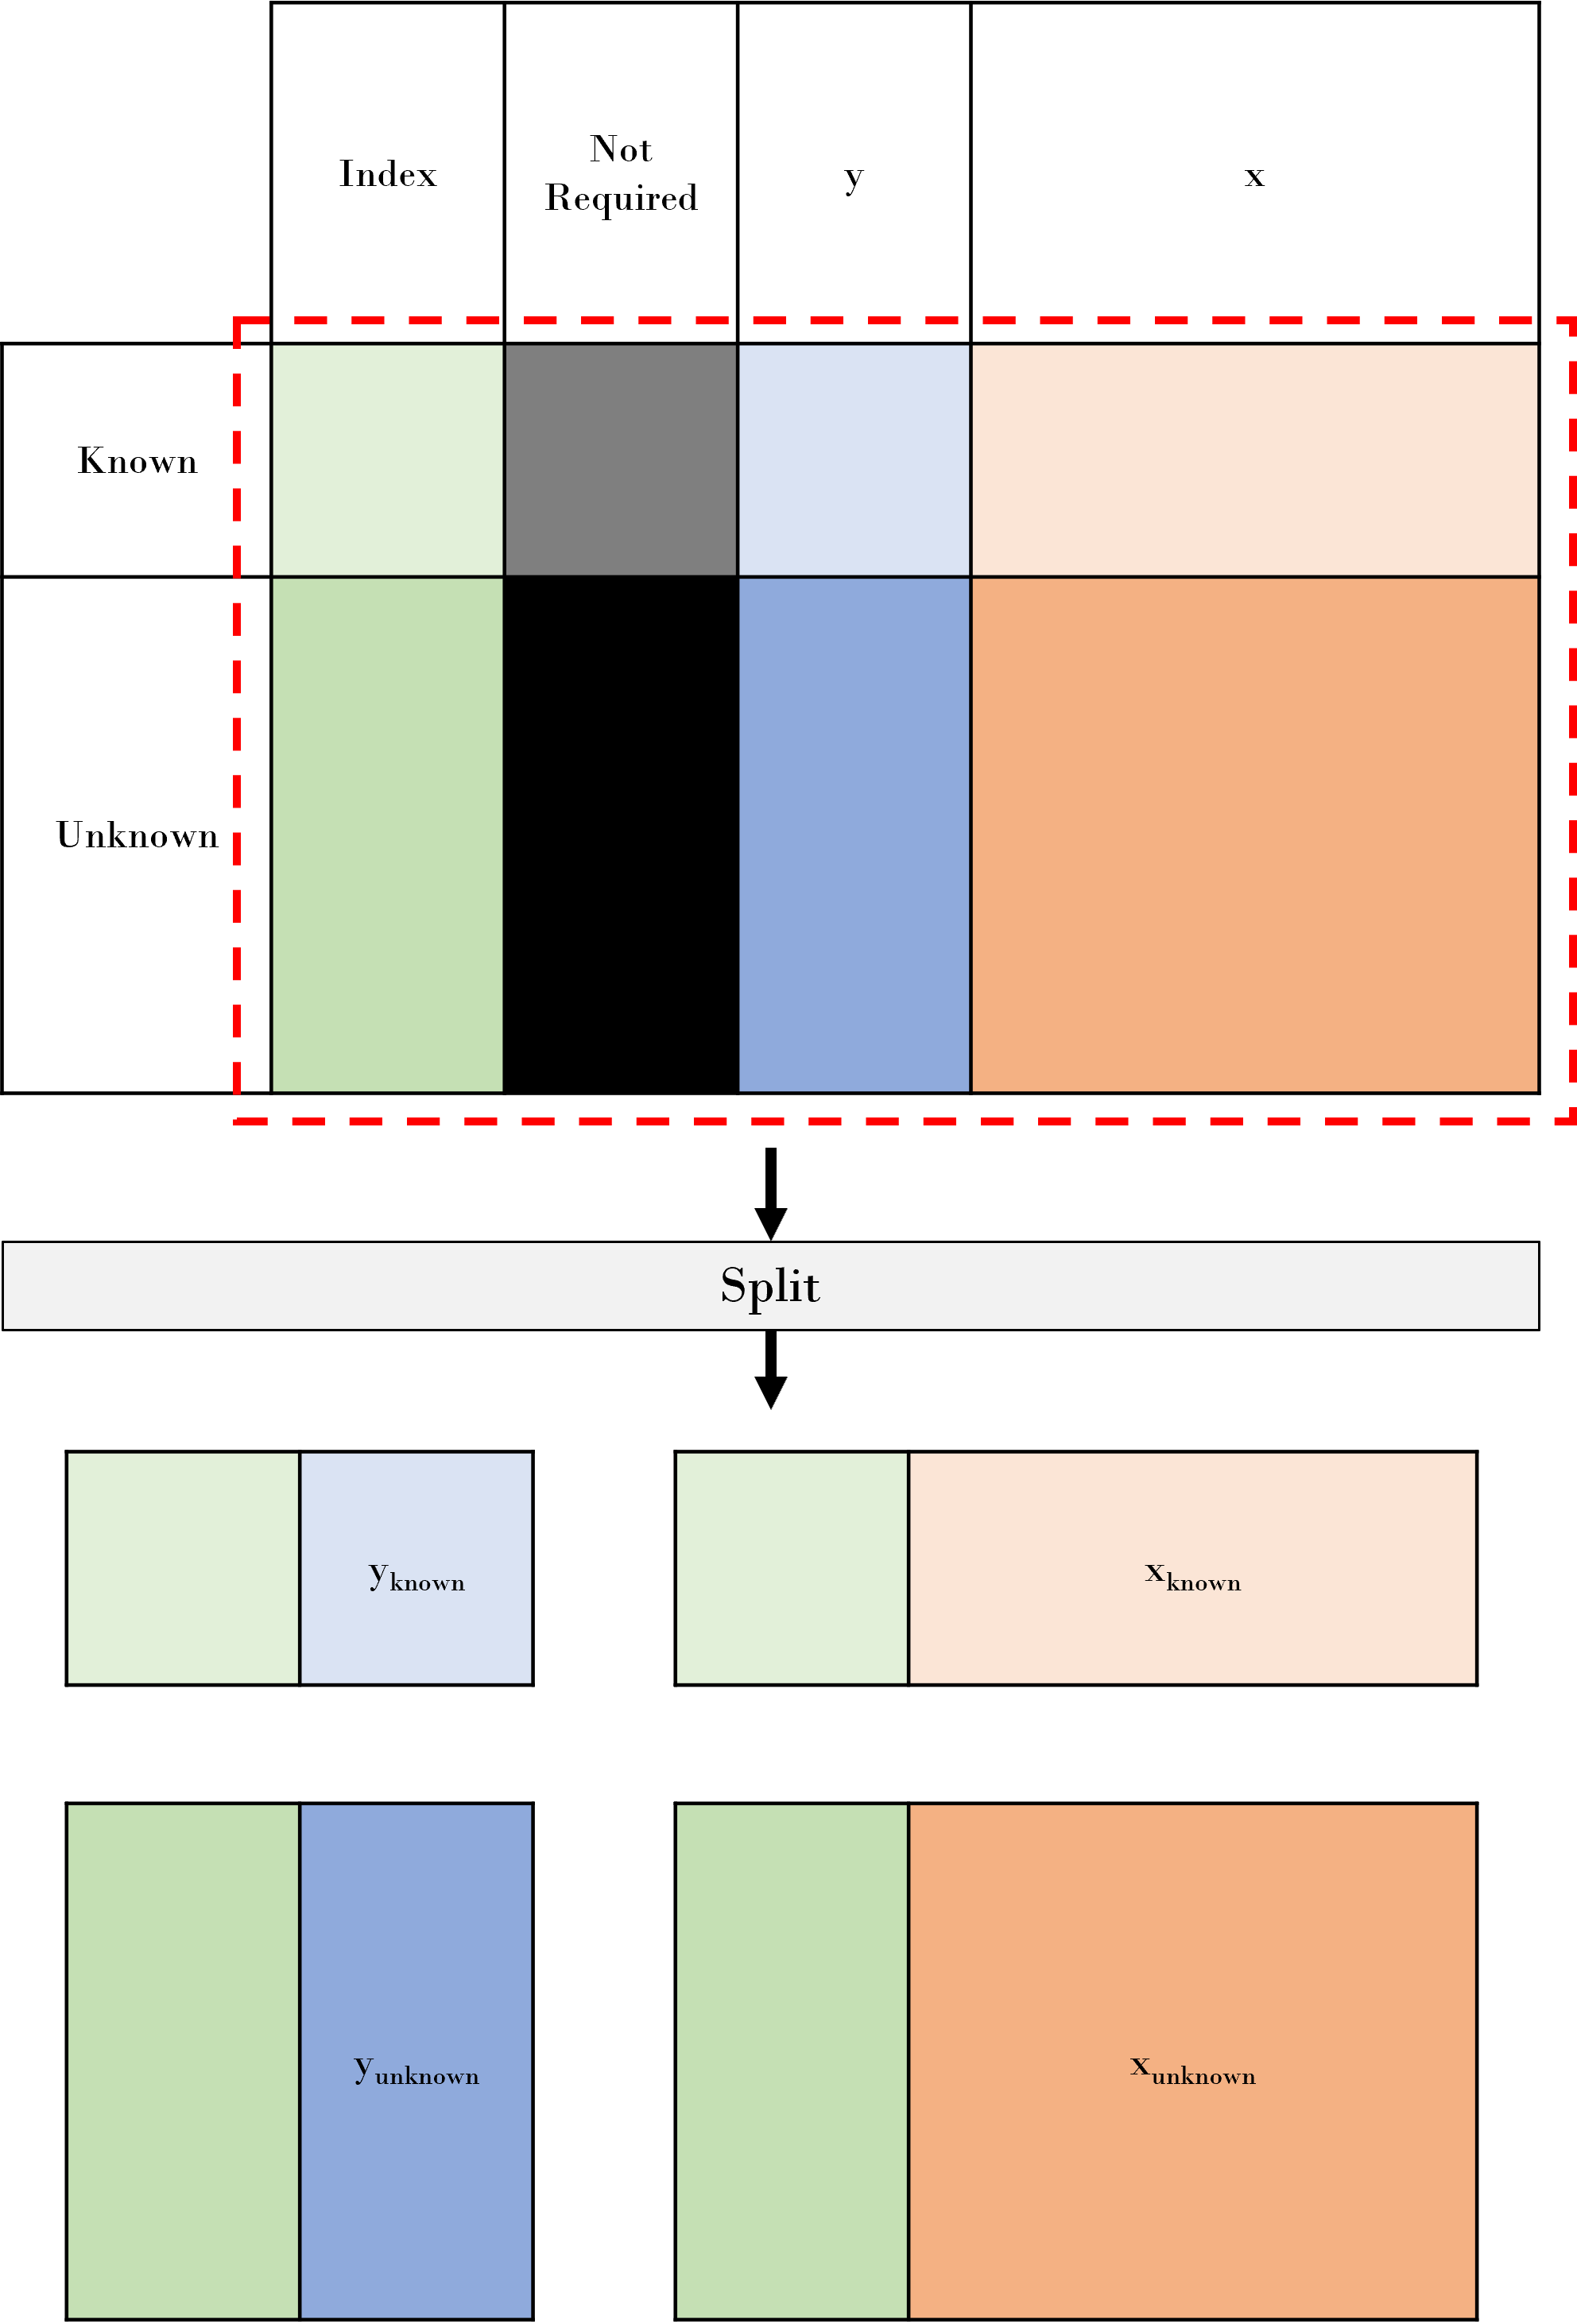
\includegraphics[width=\textwidth]{split.png}
        \end{center}
        \caption[Representation of the split function]{Graphical representation of the\lstinline{split}function. The red dashed boundary represents the input (additional colour coding has been performed to assist the reader in understanding the transposition of the base components).}
        \label{fig:Split}
    \end{figure}


    \subsubsection{\lstinline{Repartition}}
    Upon each iteration, the sets provided to the algorithms need to be repartitioned to allow for the continual operation of the algorithm. This consists of two parts: expanding the known sets and removing entries from the unknown sets.

    \subsubsection{\lstinline{Model}}
    The machine learning model is the only custom class used. Here, a similar structure is used when compared with sci-kit's machine learning \cite{scikit}, as is demonstrated in Table~\ref{tab:Model}. To manage this, it has four methods:\lstinline{__init__},\lstinline{fit},\lstinline{predict}, and\lstinline{predict_error}. The last of these is not seen in all sci-kit's machine learning models and is reserved for those which can report a certainty of prediction. Here, this was achieved by taking a standard deviation of the models.

    \begin{table}[H]
        \centering
        \begin{tabular}{@{}ccc@{}}
            \toprule
                                                   & Name                         & Description                                                                                      \\ \midrule
            Attributes                             & Models: List                 & List of models to be used in composite                                                           \\ \midrule
            \multirow{3}{*}{Methods}               & fit(X: int[][], Y: double[]) & Fits the models in Models                                                                        \\
                                                   &
            predict(X: int[][]): double[]          &
            \begin{tabular}[c]{@{}c@{}}Takes a set of labels and returns mean\\ predicted label from all the models.\end{tabular}                                                    \\
                                                   &
            predict\_error(X: int[][]): double[][] &
            \begin{tabular}[c]{@{}c@{}}Takes a set of labels and returns the mean\\ predicted label from all the models and\\ standard deviations of model predictions.\end{tabular} \\
            \bottomrule
        \end{tabular}
        \caption{Schema for the Model Class.}
        \label{tab:Model}
    \end{table}

    The models used for the composite model were \dots which will be consistent across all algorithms. This allows direct comparison of the algorithms without interference from machine learning models used.

    \subsubsection{\lstinline{Validate}}
    This method implements a weighted mean squared error ($\mathrm{wmse}$) given in \ref{eq:wmse} where $w$ is given as a normalisation of the true label such that $\sum{w}=1$ and ${0\leq{}w\leq{}1}$. Further modification to this ensures the base case with five data points provides a $\mathrm{wmse}=1$ and the score if the entire dataset is modelled provides a $\mathrm{wmse}=0$.

    \begin{equation}
        \mathrm{wmse}=\frac{1}{n}\sum_{i=0}^{n-1}{w_i(y_i-\bar{y})^2}
        \label{eq:wmse}
    \end{equation}

    This achieves several goals. Firstly, it targets the higher values of pChEMBL, as these are the most beneficial for drug development. Secondly, it reduces the natural spread in results for datasets, preventing those poorly capable of being predicted the model from displacing results from the algorithm. Finally, it allows the results to be given as a fractional improvement instead. It allows a target of "85\%" prediction to be given for stopping criteria if desired.

    \subsection{Active Learning Algorithms}

    \subsubsection{Dumb}

    The dumb algorithm, also referred to as random sampling or Monte Carlo sampling, refers to an algorithm that calls upon random samples to be tested. This represents the computationally least expensive approach, and is thus used as a baseline in comparing other algorithms. Since the datasets are shuffled prior to being used, the algorithm is extremely simple, as demonstrated in Algorithm~\ref{alg:MC}.

    \begin{algorithm}[H]
        \KwData{$X_\mathrm{unknown}$}
        \KwResult{$X$ ordered according to priority for sampling}
        \Return{$\mathrm{ones\_like}(X_\mathrm{unknown})$}
        \caption{Uncertainty Sampling Selection}
        \label{alg:MC}\SetAlgoLined
    \end{algorithm}

    \subsubsection{Greedy}
    Since the largest activity is sought, a methodology proposed is to simply seek the predicted highest label. Here, the predict() method (see Table~\ref{tab:Model}) was used to return a prediction and a standard deviation. The indices of $x_\mathrm{unknown}$ were then returned, ordered descending with respect to the afore mentioned standard deviations.

    \begin{algorithm}[H]
        \KwData{$X_\mathrm{known}$, $Y_\mathrm{known}$, $X_\mathrm{unknown}$, Model}
        \KwResult{$X$ ordered according to priority for sampling}
        Model.fit($X_\mathrm{known}$, $Y_\mathrm{known}$)\;
        prediction = Model.predict\_error($X_\mathrm{unknown}$)\;
        \Return{$-\mathrm{prediction}$}
        \caption{Greedy Sampling Selection}
        \label{alg:greedy}\SetAlgoLined
    \end{algorithm}

    \subsubsection{Region of Disagreement}
    Similarly to the region of disagreement method, this is a very simple algorithm. Here, the predict\_error() method (see Table~\ref{tab:Model}) is used to return a prediction and a standard deviation. The prediction is ignored, and instead the standard deviation is returned, multiplied by $-1$ to ensure the largest uncertainty has the lowest "score". This is shown with Algorithm~\ref{alg:rod}.

    \begin{algorithm}[H]
        \KwData{$X_\mathrm{known}$, $Y_\mathrm{known}$, $X_\mathrm{unknown}$, Model}
        \KwResult{$X$ ordered according to priority for sampling}
        Model.fit($X_\mathrm{known}$, $Y_\mathrm{known}$)\;
        \_, error = Model.predict\_error($X_\mathrm{unknown}$)\;
        \Return{$-\mathrm{error}$}
        \caption{Uncertainty Sampling Selection}
        \label{alg:rod}\SetAlgoLined
    \end{algorithm}

    \subsubsection{Hotspot Cluster I}
    This is the first of the clustering algorithms and the first parametric algorithm. This algorithm is based upon the ideology presented in Section~\ref{sec:litRevDH}, and is shown in Algorithm~\ref{alg:cluster1}. Here, $c$ is the number of cluster sought, and is a parameter that requires fitting. Bounds can be placed upon this. The lower limit can be set as the number of known data points, and the upper as the total number of data points in the data set, although it is hypothesised that beyond the sum of the known points and the samples sought would make little, to no difference. To test this hypothesis, the upper limit will be set at $\mathrm{len}(X_\mathrm{unknown})+1.5n$. The combined limits have been shown in \ref{eq:limsClust1}.

    \begin{equation}
        \label{eq:limsClust1}
        {\mathrm{len}(X_\mathrm{known})<c<\mathrm{len}(X_\mathrm{unknown})+1.5n}
    \end{equation}

    \begin{algorithm}[H]
        \KwData{$X_\mathrm{known}$, $X_\mathrm{unknown}$, $c$}
        \KwResult{$X$ ordered according to priority for sampling}
        combined\_x = concat(X, x)\;
        clusters = cluster(number\_of\_clusters=$c$)\;
        clusters.fit(combined\_x)\;
        predicted\_custers = clusters.predict($X_\mathrm{unknown}$)\;
        distances = clusters.distance\_to\_nearest\_centroid($X_\mathrm{unknown}$)\;

        \Return{$-\mathrm{error}$}
        \caption{Uncertainty Sampling Selection}
        \label{alg:cluster1}\SetAlgoLined
    \end{algorithm}

    \subsubsection{Hotspot Cluster II}
    This is similar to the previous algorithm with one difference, the labels. Both known and predicted are used within the algorithm to ...

    \subsubsection{Hotspot Cluster III}
    The final hotspot clustering algorithm also encompasses the uncertainty from the prediction models.

    \subsubsection{Region of Disagreement with Greedy Sampling}
    This is the first composite function, combining both the greedy sampling, and the uncertainty sampling algorithms. This metric is shown in \ref{eq:rodAndGreed}.

    \begin{equation}
        \label{eq:rodAndGreed}
        {\mathrm{score}_\mathrm{greedy\&uncertainty}=\mathrm{score}_\mathrm{greedy}^{\alpha}\mathrm{score}_\mathrm{uncertainty}^{1-\alpha}}
    \end{equation}

    Here, $\alpha$ is a parameter which needs to be found, bounded as $0<\alpha{}<1$. Note here that the limits are identical to the uncertainty sampling and the greedy methodologies.

    \subsection{Training Framework}
    \blindtext[1]
    \subsubsection{Parallelisation}
    The large number of datasets used presents a problem: time. Indeed, each iteration sees a new fitting of a machine learning model. Within the training stage, this would correspond to 984 models trained: a considerable number. Thus, by exploiting parallelisation, the time can be reduced in execution to the case, where given an infinite number of processes, the training and testing framework would scale as $\mathcal{O}(c)$. This requires circumventing pythons global interpreter lock. Pathos was used to accomplish this due to several shortcomings found with the default multiprocessing package \cite{pathos1,pathos2}.

\subsubsection{Minimisation}
The methodology for minimisation was dependent on the circumstance. Firstly, the range was proved viable using a grid of points within the bound suggested earlier. Upon confirmation of the bounds, a more vigarous method was used: particularly in the case where doubles could be used. In several examples, such as in Clusterisation I, the parameter used was a integer. This was minisimised through a binary search, as most available optimisers fail to adapt to integer arguments.
\blindtext[1]